\documentclass{article}
\usepackage{times}
\usepackage[utf8]{inputenc}
\usepackage[T1]{fontenc}
\usepackage[russian]{babel}
\usepackage[a4paper, total={6in, 8in}]{geometry}
\usepackage{dirtytalk}
\usepackage{graphicx}
\usepackage{hyperref}
\usepackage{listings}
\usepackage{color,soul}
\usepackage{xcolor}

\graphicspath{ {./img/} }

% code listings settings
\definecolor{lightgray}{rgb}{.9,.9,.9}
\definecolor{darkgray}{rgb}{.4,.4,.4}
\definecolor{purple}{rgb}{0.65, 0.12, 0.82}

\lstdefinelanguage{JavaScript}{
	keywords={break, case, catch, continue, debugger, default, delete, do, else, false, finally, for, function, if, in, instanceof, new, null, return, switch, this, throw, true, try, typeof, var, void, while, with},
	morecomment=[l]{//},
	morecomment=[s]{/*}{*/},
	morestring=[b]',
	morestring=[b]",
	ndkeywords={class, export, boolean, throw, implements, import, this},
	keywordstyle=\color{blue}\bfseries,
	ndkeywordstyle=\color{darkgray}\bfseries,
	identifierstyle=\color{black},
	commentstyle=\color{purple}\ttfamily,
	stringstyle=\color{red}\ttfamily,
	sensitive=true
}

\lstset{
	language=JavaScript,
	backgroundcolor=\color{lightgray},
	columns=fullflexible,
	basicstyle=\ttfamily,
	extendedchars=false,
	showstringspaces=false,
	showspaces=false,
	numbers=left,
	numberstyle=\footnotesize,
	numbersep=9pt,
	tabsize=2,
	breaklines=true,
	showtabs=false,
	captionpos=b
}


\begin{document}
	

\textcolor{red}{{\huge **BETA VERSION, NEED FULL REVIEW AND REFACTOR**}}
	
\title{Лабораторная работа 1}

\date{\today}
\maketitle

\say{Когда кто-то говорит: «Я хочу язык программирования, который может делать все, что ему скажу», то я даю этому человеку леденец.
	— Alan J. Perlis}

\section{Введение}

Цель: изучить структуру и работу BlockChain


\section{Основные понятия}


\begin{itemize}
	\item BlockChain (блокчейн) - выстроенная по определённым правилам непрерывная последовательная цепочка блоков (связный список), содержащих информацию. Чаще всего копии цепочек блоков хранятся на множестве разных компьютеров независимо друг от друга. 
	\item 
	\item 	
\end{itemize}


\section{Proof-of-work}

Основная концепция блокчейна довольно проста: распределенная база данных, которая поддерживает постоянно растущий список упорядоченных записей. 

Однако, многоe остается непонятным, если говорить о блокчейне, так же остается много проблем, которые пытаются решить с его помощью. Это относится и к популярным блокчейн проектам, таким как Биткоин (Bitcoin) и Эфириума (Ethereum). Термин "блокчейн" обычно сильно привязан к концепции типа денежных переводов, смарт-контрактов или криптовалюты. Это делает понимание блокчейна сложнее, чем есть на самом деле.

Далее будет показана реализация простого блокчейна на языке  \hl{TypeScrypt}. Он был выбран так как является очень похожим на язык \hl{Solidity}, который будет необходимо изучить для последней лабораторной.

\subsection{Структура блока}


Первый логический шаг — определиться со структурой блока. Чтобы оставить все как можно проще, включим только самое необходимое  (Рис. 1):


\begin{itemize}
\item index : Высота блока в блокчейне.
\item data: Любые данные в блоке.
\item timestamp: Временная метка.
\item hash: SHA256 текущего блока
\item previousHash: Ссылка на хеш предыдущего блока. Это зачение полностью определяет предыдущий блок.
\end{itemize}

Код такого блока выглядит таким образом:


\begin{lstlisting}[language=JavaScript, caption={Структура блока}]
class Block {

	public index: number;
	public hash: string;
	public previousHash: string;
	public timestamp: number;
	public data: string;

constructor(index: number, hash: string, previousHash: string, timestamp: number, data: string) {
	this.index = index;
	this.previousHash = previousHash;
	this.timestamp = timestamp;
	this.data = data;
	this.hash = hash;
}

}
\end{lstlisting}


\begin{figure}
	\centering
	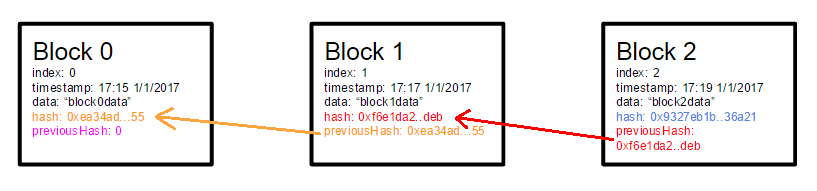
\includegraphics[scale=0.45]{blockchain_scheme}
	\caption{Структура блоков в блокчейне.}
	\label{fig:blockchain_scheme}
\end{figure}

\subsection{Хеш блока}

Хэш блока является одним из наиболее важных свойств блока. Хэш вычисляется по всем данным блока. Это означает, что если что-либо в блоке изменится, исходный хэш больше недействителен. Хэш блока также можно рассматривать как уникальный идентификатор блока. Например, могут появляться блоки с одним и тем же индексом, но все они имеют уникальные хэши.

Вычисляем хэш блока, используя следующий код:

\begin{lstlisting}[language=JavaScript, caption={Вычисление хэша блока}]
const calculateHash = (index: number, previousHash: string, timestamp: number, data: string): string =>
CryptoJS.SHA256(index + previousHash + timestamp + data).toString();
\end{lstlisting}

Следует отметить, что блок-хэш еще не имеет ничего общего с майнингом, так как нет доказательства работы (prof-of-work). Мы используем хеши блоки, чтобы сохранить целостность блока и явно ссылаться на предыдущий блок.

Важным следствием свойств hash и previousHash является то, что блок не может быть изменен без изменения хэша каждого последовательного блока.

Это показано в приведенном ниже примере. Если данные в блоке 44 изменены с «DESERT» на «STREET», все хэши предыдущих блоков должны быть изменены (Рис. 2). Это связано с тем, что хэш блока зависит от значения предыдущего Hash (между прочим).

\begin{figure}
	\centering
	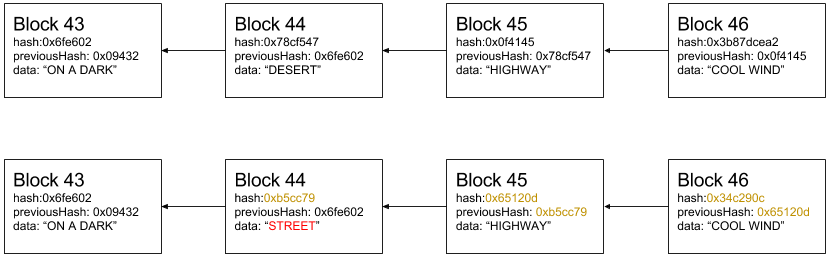
\includegraphics[scale=0.45]{previous_hash_chain}
	\caption{Зависимость хеша от данных}
	\label{fig:previous_hash_chain}
\end{figure}

Это особенно важное свойство, когда вводится proof-of-work. Чем выше блок в блочной цепочке, тем сложнее его модифицировать, так как это потребует изменений для каждого предыдущего блока.


\subsection{Генерация блока}

Чтобы сгенерировать блок, мы должны знать хэш предыдущего блока и создать остальную часть требуемого контента (индекс, хэш, данные и временную метку). Данные блока - это то, что предоставляется конечным пользователем, но остальные параметры будут сгенерированы с использованием следующего кода:


\begin{lstlisting}[language=JavaScript, caption={Генерация блока}]
const generateNextBlock = (blockData: string) => {
	const previousBlock: Block = getLatestBlock();
	const nextIndex: number = previousBlock.index + 1;
	const nextTimestamp: number = new Date().getTime() / 1000;
	const nextHash: string = calculateHash(nextIndex, previousBlock.hash, nextTimestamp, blockData);
	const newBlock: Block = new Block(nextIndex, nextHash, previousBlock.hash, nextTimestamp, blockData);
	return newBlock;
};
\end{lstlisting}

\subsection{Хранение блоков}

В памяти массив JavaScript используется для хранения блокчейн. Первый блок в блокчейн — это всегда так называемый «генезис-блок», имеющий следующий код:

\begin{lstlisting}[language=JavaScript, caption={Хранение блоков}]
const blockchain: Block[] = [genesisBlock];
\end{lstlisting}


\subsection{Проверка целостности блоков}

В любой момент времени мы должны иметь возможность проверить, действителен ли блок или цепочка блоков с точки зрения целостности. Это верно, особенно когда мы получаем новые блоки от других узлов и должны решить, принимать их или нет.

Чтобы блок был действительным, необходимо применить следующее:

\begin{itemize}
	\item Индекс блока должен быть на один номер больше предыдущего.
	\item \hl{previusHash} блока соответствует \hl{hash} предыдущего блока.
	\item \hl{hash} самого блока должен быть действительным.
\end{itemize}

Это демонстрируется следующим кодом:


\begin{lstlisting}[language=JavaScript, caption={Проверка целостности блоков}]
const isValidNewBlock = (newBlock: Block, previousBlock: Block) => {
	if (previousBlock.index + 1 !== newBlock.index) {
		console.log('invalid index');
		return false;
	} else if (previousBlock.hash !== newBlock.previousHash) {
		console.log('invalid previoushash');
		return false;
	} else if (calculateHashForBlock(newBlock) !== newBlock.hash) {
		console.log(typeof (newBlock.hash) + ' ' + typeof calculateHashForBlock(newBlock));
		console.log('invalid hash: ' + calculateHashForBlock(newBlock) + ' ' + newBlock.hash);
		return false;
	}
	return true;
};
\end{lstlisting}

Мы также должны проверить структуру блока, чтобы искаженный контент, отправленный одноранговым узлом, не разбивал наш узел.

\begin{lstlisting}[language=JavaScript, caption={Проверка полей структуры блока}]
const isValidBlockStructure = (block: Block): boolean => {
	return typeof block.index === 'number'
		&& typeof block.hash === 'string'
		&& typeof block.previousHash === 'string'
		&& typeof block.timestamp === 'number'
		&& typeof block.data === 'string';
};
\end{lstlisting}

Теперь, когда у нас есть средства для проверки одного блока, мы можем перейти к проверке полной цепочки блоков. Сначала мы проверим, что первый блок в цепочке совпадает с \hl{genesisBlock}. После этого мы проверяем каждый последовательный блок с использованием ранее описанных методов. Это демонстрируется следующим кодом:

\begin{lstlisting}[language=JavaScript, caption={Проверка полей структуры блока}]
const isValidChain = (blockchainToValidate: Block[]): boolean => {
	const isValidGenesis = (block: Block): boolean => {
		return JSON.stringify(block) === JSON.stringify(genesisBlock);
	};
	
	if (!isValidGenesis(blockchainToValidate[0])) {
		return false;
	}
	
	for (let i = 1; i < blockchainToValidate.length; i++) {
		if (!isValidNewBlock(blockchainToValidate[i], blockchainToValidate[i - 1])) {
			return false;
		}
	}
	return true;
};
\end{lstlisting}


\subsection{Выбор самый длинной цепочки блоков}

Всегда должен быть только один явный набор блоков в цепочке в данный момент времени. В случае конфликтов (например, два узла генерируют номер блока 72), мы выбираем цепочку с самым длинным числом блоков. В приведенном ниже примере данные (Рис. 3), введенные в блоке 72: a350235b00, не будут включены в цепочку блоков, поскольку она будет переопределена более длинной цепочкой.

\begin{figure}
	\centering
	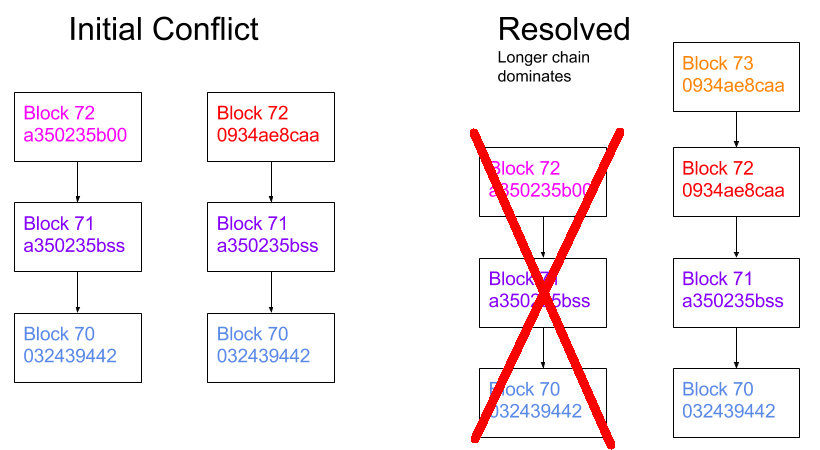
\includegraphics[scale=0.35]{conflict_resolving}
	\caption{Конфликт цепочек}
	\label{fig:conflict_resolving}
\end{figure}

Это логика реализована с использованием следующего кода:


\begin{lstlisting}[language=JavaScript, caption={Выбор самой длинной цепочки блоков}]
const replaceChain = (newBlocks: Block[]) => {
	if (isValidChain(newBlocks) && newBlocks.length > getBlockchain().length) {
		console.log('Received blockchain is valid. Replacing current blockchain with received blockchain');
		blockchain = newBlocks;
		broadcastLatest();
	} else {
		console.log('Received blockchain invalid');
	}
};
\end{lstlisting}


\subsection{Работа с узлами сети}

Существенной частью узла является совместное использование и синхронизация блочной цепи с другими узлами. Следующие правила используются для синхронизации сети(Рис. 4).

\begin{itemize}
	\item Когда узел генерирует новый блок, он передает его в сеть.
	\item Когда узел соединяется с новым одноранговым узлом, он запрашивает последний блок.
	\item Когда узел встречает блок с индексом, большим, чем текущий известный блок, он либо добавляет блок своей текущей цепочке, либо запросы для полной блок-цепи.
\end{itemize}


\begin{figure}
	\centering
	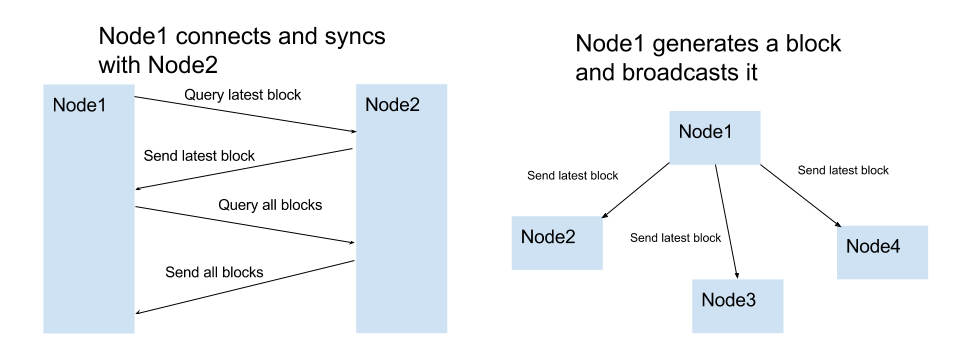
\includegraphics[scale=0.4]{p2p_communication}
	\caption{Конфликт цепочек}
	\label{fig:p2p_communication}
\end{figure}


Мы будем использовать websockets для одноранговой связи. Активные сокеты для каждого узла хранятся в переменной \hl{const sockets: WebSocket []}. Автоматическое обнаружение одноранговых сетей не используется. Места расположения (= URL-адреса веб-узлов) пиров должны быть добавлены вручную.

\subsection{Управление узлом}

Пользователь должен иметь возможность управлять узлом каким-либо образом. Это делается путем настройки HTTP-сервера.

\begin{lstlisting}[language=JavaScript, caption={Управление узлом сети}]
const initHttpServer = ( myHttpPort: number ) => {
	const app = express();
	app.use(bodyParser.json());
	
	app.get('/blocks', (req, res) => {
		res.send(getBlockchain());
	});
	app.post('/mineBlock', (req, res) => {
		const newBlock: Block = generateNextBlock(req.body.data);
		res.send(newBlock);
	});
	app.get('/peers', (req, res) => {
		res.send(getSockets().map(( s: any ) => s._socket.remoteAddress + ':' + s._socket.remotePort));
	});
	app.post('/addPeer', (req, res) => {
		connectToPeers(req.body.peer);
		res.send();
	});
	
	app.listen(myHttpPort, () => {
		console.log('Listening http on port: ' + myHttpPort);
	});
};
\end{lstlisting}


Как видно, пользователь может взаимодействовать с узлом следующими способами:

\begin{itemize}
	\item Получить список всех блоков.
	\item Создать новый блок с заданным содержимым.
	\item Вывести или добавить пиров. 
\end{itemize}

Наиболее простым способом управления узлом является, например, с \hl{Curl}:

\begin{lstlisting}[caption={Отправка HTTP запроса, для получения списка блоков.}]
$ curl http://localhost:3001/blocks
\end{lstlisting}


\subsection{Архитектура}

Следует отметить, что узел фактически предоставляет два веб-сервера: один для пользователя для управления узлом (HTTP-сервер) и один для одноранговой связи между узлами. (HTTP-сервер Websocket)

\begin{figure}
	\centering
	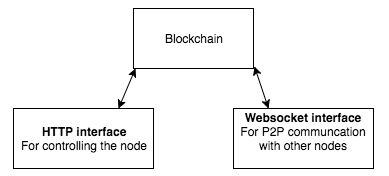
\includegraphics[scale=0.5]{architecture}
	\caption{Архитектура.}
	\label{fig:architecture}
\end{figure}

\section{Транзакции}

\subsection{Криптография на открытых ключах и подпись}

В криптографии с открытым ключом у вас есть ключевая пара: секретный ключ и открытый ключ. Открытый ключ может быть получен из секретного ключа, но секретный ключ не может быть получен из открытого ключа. Открытый ключ (как следует из названия) может быть безопасно передан всем.

Любые сообщения могут быть подписаны с использованием закрытого ключа для создания подписи. С помощью этой подписи и соответствующего открытого ключа каждый может проверить, что подпись создается секретным ключом, который соответствует открытому ключу (Рис. 6).

\begin{figure}
	\centering
	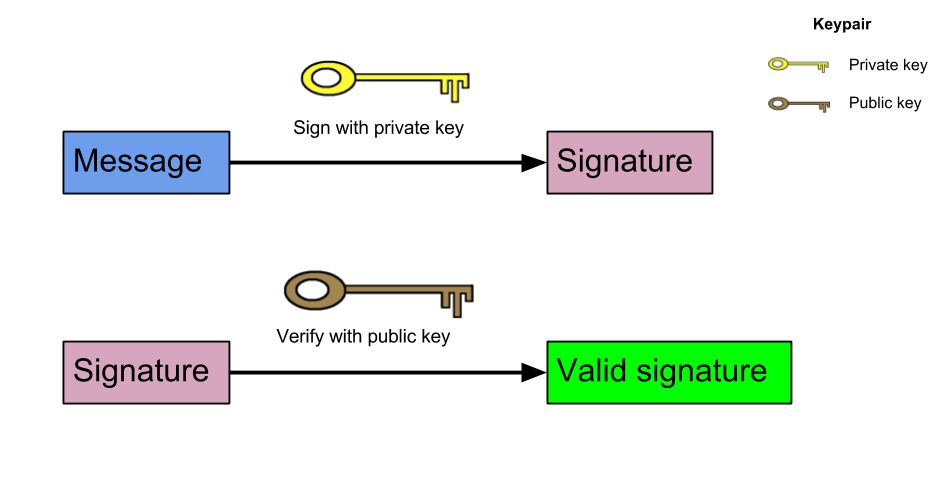
\includegraphics[scale=0.45]{signature}
	\caption{Подпись с использованием открытого и закрытого ключа.}
	\label{fig:signature}
\end{figure}

Мы будем использовать библиотеку, называемую \href{https://github.com/indutny/elliptic}{elliptic} для криптографии с открытым ключом, которая использует эллиптические кривые. \href{https://en.wikipedia.org/wiki/Elliptic_Curve_Digital_Signature_Algorithm}{ECDSA}

В криптовалютах для разных целей используются две разные криптографические функции:
\begin{itemize}
	\item Хеш-функция (SHA256) для интеллектуального анализа (хэш также используется для сохранения целостности блока).
	\item Криптография с открытым ключом (ECDSA) для транзакций.
\end{itemize}

\subsection{Открытые и закрытые ключи в ECDSA}

Допустимым закрытым ключом является любая случайная 32-байтовая строка, например:
 
\begin{lstlisting}
19f128debc1b9122da0635954488b208b829879cf13b3d6cac5d1260c0fd967c
\end{lstlisting}
Допустимым открытым ключом является "04", объединенный с 64-байтовой строкой, например: 

\begin{lstlisting}
 04bfcab8722991ae774db48f934ca79cfb7dd991229153b9f732ba5334aafcd8e7266e47076996b55
 a14bf9913ee3145ce0cfc1372ada8ada74bd287450313534a
\end{lstlisting}

Открытый ключ можно получить из закрытого ключа. Открытый ключ будет использоваться как "получатель" (адрес) монет в транзакции.

\subsection{Знакомство с транзакциями}

Прежде чем писать код, давайте рассмотрим структуру транзакций. Транзакции состоят из двух компонентов: вводы и выводы. В выводе указывается, куда отправляются монеты, а ввод дает доказательство того, что монеты, которые действительно отправлены, существуют и в первую очередь и принадлежат "отправителю". Вводы всегда относятся к существующему выводу (Рис. 7).

\begin{figure}
	\centering
	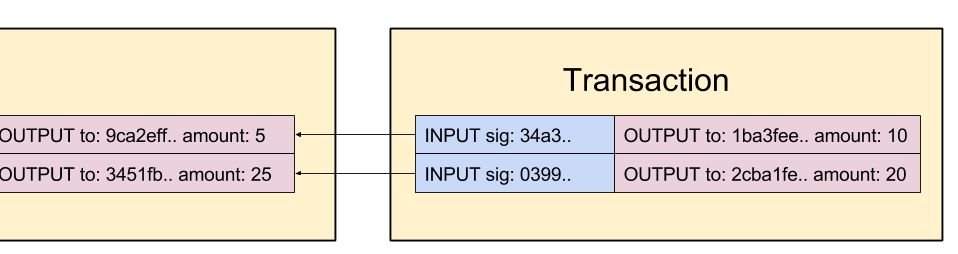
\includegraphics[scale=0.45]{transactions}
	\caption{Структура транзакции.}
	\label{fig:transactions}
\end{figure}

\subsection{Выводы транзакций}

Выводы транзакции \hl{txOut} состоят из адреса и количества монет. Адрес является открытым ключом ECDSA. Это означает, что пользователь, имеющий закрытый ключ ссылочного открытого ключа (адрес), сможет получить доступ к монетам.

\begin{lstlisting}[language=JavaScript, caption={Класс вывода транзакции.}]
class TxOut {
	public address: string;
	public amount: number;
	
	constructor(address: string, amount: number) {
		this.address = address;
		this.amount = amount;
	}
}
\end{lstlisting}

\subsection{Вводы транзакций}

Вводы транзакций \hl{txIn} предоставляют информацию "откуда" монеты. Каждый \hl{txIn} ссылается на более ранний вывод, из которого монеты «разблокированы», с подписью. Эти разблокированные монеты теперь доступны для \hl{txOut}. Подпись дает доказательство того, что только пользователь, имеющий закрытый ключ упомянутого открытого ключа (адрес), мог создать транзакцию.

\begin{lstlisting}[language=JavaScript, caption={Класс вводы транзакции.}]
class TxIn {
	public txOutId: string;
	public txOutIndex: number;
	public signature: string;
}
\end{lstlisting}

Следует отметить, что \hl{txIn} содержит только подпись (созданную закрытым ключом), а не сам закрытый ключ. Блок-цепочка содержит открытые ключи и подписи, а не закрытые ключи.

Можно также представить, что \hl{txIn} разблокирует монеты, а \hl{txOuts} заблокирует их обратно (Рис 8):

\begin{figure}
	\centering
	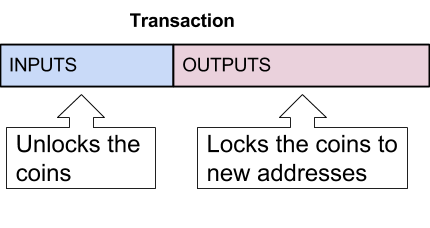
\includegraphics[scale=0.45]{trans_lock}
	\caption{Вводы и выводы.}
	\label{fig:trans_lock}
\end{figure}

\subsection{Класс транзакции}

Сама структура транзакций довольно проста, так как теперь мы определили \hl{txIns} и \hl{txOuts}.

\begin{lstlisting}[language=JavaScript, caption={Класс транзакции.}]
class Transaction {
	public id: string;
	public txIns: TxIn[];
	public txOuts: TxOut[];
}
\end{lstlisting}

\subsection{Идентификатор транзакции}

Идентификатор транзакции рассчитывается путем принятия хеша из содержимого транзакции. Однако подписи \hl{txIds} не включаются в хэш транзакции, поскольку они будут добавлены позже к транзакции.

\begin{lstlisting}[language=JavaScript, caption={Генерирование идентификатора транзакции.}]
const getTransactionId = (transaction: Transaction): string => {
	const txInContent: string = transaction.txIns
		.map((txIn: TxIn) => txIn.txOutId + txIn.txOutIndex)
		.reduce((a, b) => a + b, '');
	
	const txOutContent: string = transaction.txOuts
		.map((txOut: TxOut) => txOut.address + txOut.amount)
		.reduce((a, b) => a + b, '');
	
	return CryptoJS.SHA256(txInContent + txOutContent).toString();
};
\end{lstlisting}

\subsection{Подпись транзакции}

Важно, чтобы содержимое транзакции не могло быть изменено после его подписания. Поскольку транзакции являются общедоступными, каждый может получить доступ к транзакциям, даже до того, как они будут включены в блок-цепочку.

При подписании транзакционных входов будет подписан только \hl{txId}. Если какое-либо содержимое в транзакции изменено, \hl{txId} должен измениться, что делает транзакцию и подпись недопустимыми.

\begin{lstlisting}[language=JavaScript, caption={Подписание входа транзакции.}]
const signTxIn = (transaction: Transaction, txInIndex: number,
	privateKey: string, aUnspentTxOuts: UnspentTxOut[]): string => {
	
	const txIn: TxIn = transaction.txIns[txInIndex];
	const dataToSign = transaction.id;
	const referencedUnspentTxOut: UnspentTxOut = findUnspentTxOut(txIn.txOutId, txIn.txOutIndex, aUnspentTxOuts);
	const referencedAddress = referencedUnspentTxOut.address;
	const key = ec.keyFromPrivate(privateKey, 'hex');
	const signature: string = toHexString(key.sign(dataToSign).toDER());
	return signature;
};
\end{lstlisting}

Попробуем понять, что произойдет, если кто-то попытается изменить транзакцию:

\begin{enumerate}
	\item  Атакующий запускает узел и получает транзакцию с контентом: «отправьте 10 монет с адреса AAA на BBB» с txId 0x555 ..
	\item Злоумышленник изменяет адрес получателя на CCC и передает его по сети в сети. Теперь содержимое транзакции «отправить 10 монет с адреса AAA в CCC»
	\item Однако, когда адрес получателя изменен, txId больше недействителен. Новый действительный txId будет 0x567 ...
	\item Если значение txId установлено на новое значение, подпись недействительна. Подпись соответствует только оригинальному txId 0x555 ..
	\item Модифицированная транзакция не будет приниматься другими узлами, поскольку в любом случае она недействительна.
\end{enumerate}

\subsection{Неизрасходованные выходы транзакций}

Вход транзакции должен всегда ссылаться на неизрасходованные выход транзакции (uTxO). Следовательно, когда вы владеете некоторыми монетами в блокчейне, то, что у вас есть на самом деле, это список неизрасходованных выходов транзакции, открытый ключ которых соответствует вашему закрытому ключу.

Что касается проверки транзакций, мы можем сосредоточиться только на списке выводов нерассмотренных транзакций, чтобы выяснить, действительна ли транзакция. Список неизрасходованных выходов транзакций всегда можно вывести из текущей блок-цепи. В этой реализации мы будем обновлять список неизрасходованных выходов транзакций при обработке и включении транзакций в цепочку.

Структура данных для неизрасходованного вывода транзакций выглядит следующим образом:

\begin{lstlisting}[language=JavaScript, caption={Класс неиспользованноых выходов.}]
class UnspentTxOut {
	public readonly txOutId: string;
	public readonly txOutIndex: number;
	public readonly address: string;
	public readonly amount: number;
	
	constructor(txOutId: string, txOutIndex: number, address: string, amount: number) {
		this.txOutId = txOutId;
		this.txOutIndex = txOutIndex;
		this.address = address;
		this.amount = amount;
	}
}
\end{lstlisting}

Сама структура даных это просто список обьектов \hl{UnspentTxOut}:


\begin{lstlisting}[language=JavaScript]
let unspentTxOuts: UnspentTxOut[] = [];
\end{lstlisting}


\subsection{Обновление неизрасходованных транзакционных выходов}

Каждый раз, когда в блокчейн добавляется новый блок, мы должны обновлять наш список неизрасходованных выходов транзакции. Это связано с тем, что новые транзакции будут тратить некоторые из существующих транзакционных выходов и внедрять новые неизрасходованные выходы.

Чтобы сделать это, мы сначала извлечем из нового блока все новые неиспользованные выходы транзакции (newUnspentTxOuts):




\begin{lstlisting}[language=JavaScript]
const newUnspentTxOuts: UnspentTxOut[] = newTransactions
	.map((t) => {
		return t.txOuts.map((txOut, index) => new UnspentTxOut(t.id, index, txOut.address, txOut.amount));
	})
	.reduce((a, b) => a.concat(b), []);
\end{lstlisting}

Мы также должны знать, какие выходы транзакции используются для создания новой транзакции (consumedTxOuts). Это будет решаться путем изучения входов новых транзакций:

\begin{lstlisting}[language=JavaScript]
const consumedTxOuts: UnspentTxOut[] = newTransactions
	.map((t) => t.txIns)
	.reduce((a, b) => a.concat(b), [])
	.map((txIn) => new UnspentTxOut(txIn.txOutId, txIn.txOutIndex, '', 0));

\end{lstlisting}

Наконец, мы можем генерировать новые неиспользованные транзакционные выходы, удаляя consumedTxOuts и добавляя newUnspentTxOuts к нашим существующим выводам транзакций.

\begin{lstlisting}[language=JavaScript]
const resultingUnspentTxOuts = aUnspentTxOuts
	.filter(((uTxO) => !findUnspentTxOut(uTxO.txOutId, uTxO.txOutIndex, consumedTxOuts)))
	.concat(newUnspentTxOuts);
\end{lstlisting}

Описанный код и функциональность содержатся в методе updateUnspentTxOuts. Следует отметить, что этот метод вызывается только после того, как транзакции в блоке (и самом блоке) были проверены.


\section{Проверка транзакций}

Теперь мы можем, наконец, изложить правила, которые делают транзакцию действительной:

\subsection{Правильная структура транзакции}

Транзакция должна соответствовать определенным классам Transaction, TxIn и TxOut

\begin{lstlisting}[language=JavaScript, caption={Проверка структуры транзакции.}]
const isValidTransactionStructure = (transaction: Transaction) => {
	if (typeof transaction.id !== 'string') {
	console.log('transactionId missing');
	return false;
	}
	...
	//check also the other members of class
}
\end{lstlisting}

Идентификатор транзакции должен быть правильно рассчитан.

\begin{lstlisting}[language=JavaScript, caption={Проверка идентификатора транзакции.}]
if (getTransactionId(transaction) !== transaction.id) {
	console.log('invalid tx id: ' + transaction.id);
	return false;
}
\end{lstlisting}

Подписи в txIns должны быть действительными, а выходы, на которые ссылаются, не должны быть использованы.

\begin{lstlisting}[language=JavaScript, caption={Проверка входов транзакции.}]
const validateTxIn = (txIn: TxIn, transaction: Transaction, aUnspentTxOuts: UnspentTxOut[]): boolean => {
	const referencedUTxOut: UnspentTxOut =
		aUnspentTxOuts.find((uTxO) => uTxO.txOutId === txIn.txOutId && uTxO.txOutId === txIn.txOutId);
	if (referencedUTxOut == null) {
		console.log('referenced txOut not found: ' + JSON.stringify(txIn));
		return false;
	}
	const address = referencedUTxOut.address;
	
	const key = ec.keyFromPublic(address, 'hex');
	return key.verify(transaction.id, txIn.signature);
};
\end{lstlisting}

Суммы значений, указанных в выходах, должны быть равны суммам значений, указанных на входах. Если вы ссылаетесь на вывод, содержащий 50 монет, сумма значений на новых выходах также должна составлять 50 монет.

\begin{lstlisting}[language=JavaScript, caption={Проверка выходов транзакции.}]
const totalTxInValues: number = transaction.txIns
	.map((txIn) => getTxInAmount(txIn, aUnspentTxOuts))
	.reduce((a, b) => (a + b), 0);

const totalTxOutValues: number = transaction.txOuts
	.map((txOut) => txOut.amount)
	.reduce((a, b) => (a + b), 0);

if (totalTxOutValues !== totalTxInValues) {
	console.log('totalTxOutValues !== totalTxInValues in tx: ' + transaction.id);
	return false;
}
\end{lstlisting}


\subsection{Транзакция - база монет}

Входы транзакций должны всегда ссылаться на неизрасходованные выходы транзакции, но откуда взялись исходные монеты в блок-цепочку? Чтобы решить эту проблему, вводится специальный тип транзакции: транзакция \hl{coinbase}

Транзакция coinbase содержит только выход, но не содержит входных данных. Это означает, что транзакция с монетами добавляет новые монеты в обращение. Мы определяем объем выпуска монетной базы 50 монет.


\begin{lstlisting}[language=JavaScript]
const COINBASE_AMOUNT: number = 50;
\end{lstlisting}

Транзакция coinbase всегда является первой транзакцией в блоке, и она включается майнером блока. Награда за монетную базу выступает в качестве стимула для майнеров: если вы найдете блок, вы сможете собрать 50 монет.

Мы добавим высоту блока для ввода транзакции базу монет. Это гарантирует, что каждая транзакция coinbase имеет уникальный txId. Без этого правила, например, транзакция с монетной базой, содержащая "дать 50 монет для адреса 0xabc", всегда будет иметь одинаковый txId.

Валидация транзакции с коинбазой немного отличается от проверки "нормальной" транзакции:

\begin{lstlisting}[language=JavaScript, caption={Проверка транзакции coinbase.}]
const validateCoinbaseTx = (transaction: Transaction, blockIndex: number): boolean => {
	if (getTransactionId(transaction) !== transaction.id) {
		console.log('invalid coinbase tx id: ' + transaction.id);
		return false;
	}
	if (transaction.txIns.length !== 1) {
		console.log('one txIn must be specified in the coinbase transaction');
		return;
	}
	if (transaction.txIns[0].txOutIndex !== blockIndex) {
		console.log('the txIn index in coinbase tx must be the block height');
		return false;
	}
	if (transaction.txOuts.length !== 1) {
		console.log('invalid number of txOuts in coinbase transaction');
		return false;
	}
	if (transaction.txOuts[0].amount != COINBASE_AMOUNT) {
		console.log('invalid coinbase amount in coinbase transaction');
		return false;
	}
	return true;
};
\end{lstlisting}

\begin{thebibliography}{9}

	\bibitem{lamport94}
	  \emph{}

\end{thebibliography}

\end{document}